
\subsubsection{補正手法の設計}


PDRによる軌跡の補正には,様々なアプローチが存在する.
複数の補正手法を統合的に扱うため,本ライブラリではTrajectoryCorrector
クラスを提供している.図\ref{fig:corrector-class}にTrajectoryCorrectorsのクラス構成を示す.
補正処理はTrajectoryCorrector,DriftCorrector,MapMatcher,BLECorrectorの4つの主要なクラスによって構成されている.

TrajectoryCorrectorは補正処理の中核となるクラスであり,他の補正クラスを
統括する役割を持つ.このクラスはBuilderパターンを採用しており,これにより
複雑なオブジェクト生成プロセスをシンプルなインターフェースで提供している.
具体的には,with\_floor\_map()やwith\_ble\_data()などのメソッドチェーンにより,
必要な補正手法を直感的に指定できる.これは特に,利用可能な環境情報が
状況によって異なる場合に有用である.例えば,フロアマップのみが利用可能な
環境では,以下のようにMapMatcherによる補正のみを指定できる:
% TODO:2.クラス単体でも使用できることを主張してもいいかも

\begin{lstlisting}
corrector = TrajectoryCorrector.builder(pdr_estimator)
    .with_floor_map(floor_map)
    .build()
\end{lstlisting}

また,BLEビーコンも利用可能な場合は,以下のように両方の補正を指定できる:

\begin{lstlisting}
corrector = TrajectoryCorrector.builder(pdr_estimator)
    .with_floor_map(floor_map)
    .with_ble_data(ble_scans, beacon_positions)
    .build()
\end{lstlisting}


図\ref{fig:corrector-sequence}は実際の使用例を示している.利用者は
TrajectoryCorrectorsBuilderを通じて必要な補正手法を指定し,build
メソッドによってTrajectoryCorrectorのインスタンスを生成する.その後,
estimate\_and\_correct\_trajectoryメソッドを呼び出し,指定された
補正手法が順次適用され,最終的な補正軌跡が得られる.
% TODO: 2.whyがない○○しました.の後の何故の部分がない
この設計により,環境に応じて適切な補正手法を選択できるだけでなく,
将来的な拡張性も確保されている.例えば,新たに磁気フィンガー
プリントを用いた補正手法を追加する場合,以下の手順で実装できる:

\begin{enumerate}
  \item MagneticCorrectorクラスを新規作成し,補正のロジックを実装
  \item TrajectoryCorrectorsBuilderにwith\_magnetic\_data()メソッドを追加
  \item TrajectoryCorrectorにMagneticCorrectorを組み込む
\end{enumerate}

この際,既存の補正クラス(DriftCorrector,MapMatcherなど)のコードは
一切変更する必要がない.これは各補正クラスが独立して実装されており,
TrajectoryCorrectorを介して緩やかに結合されているためである.
% TODO: 2.このあたりいらないか,修正する必要があるかも?

\begin{figure}[H]
    \centering
    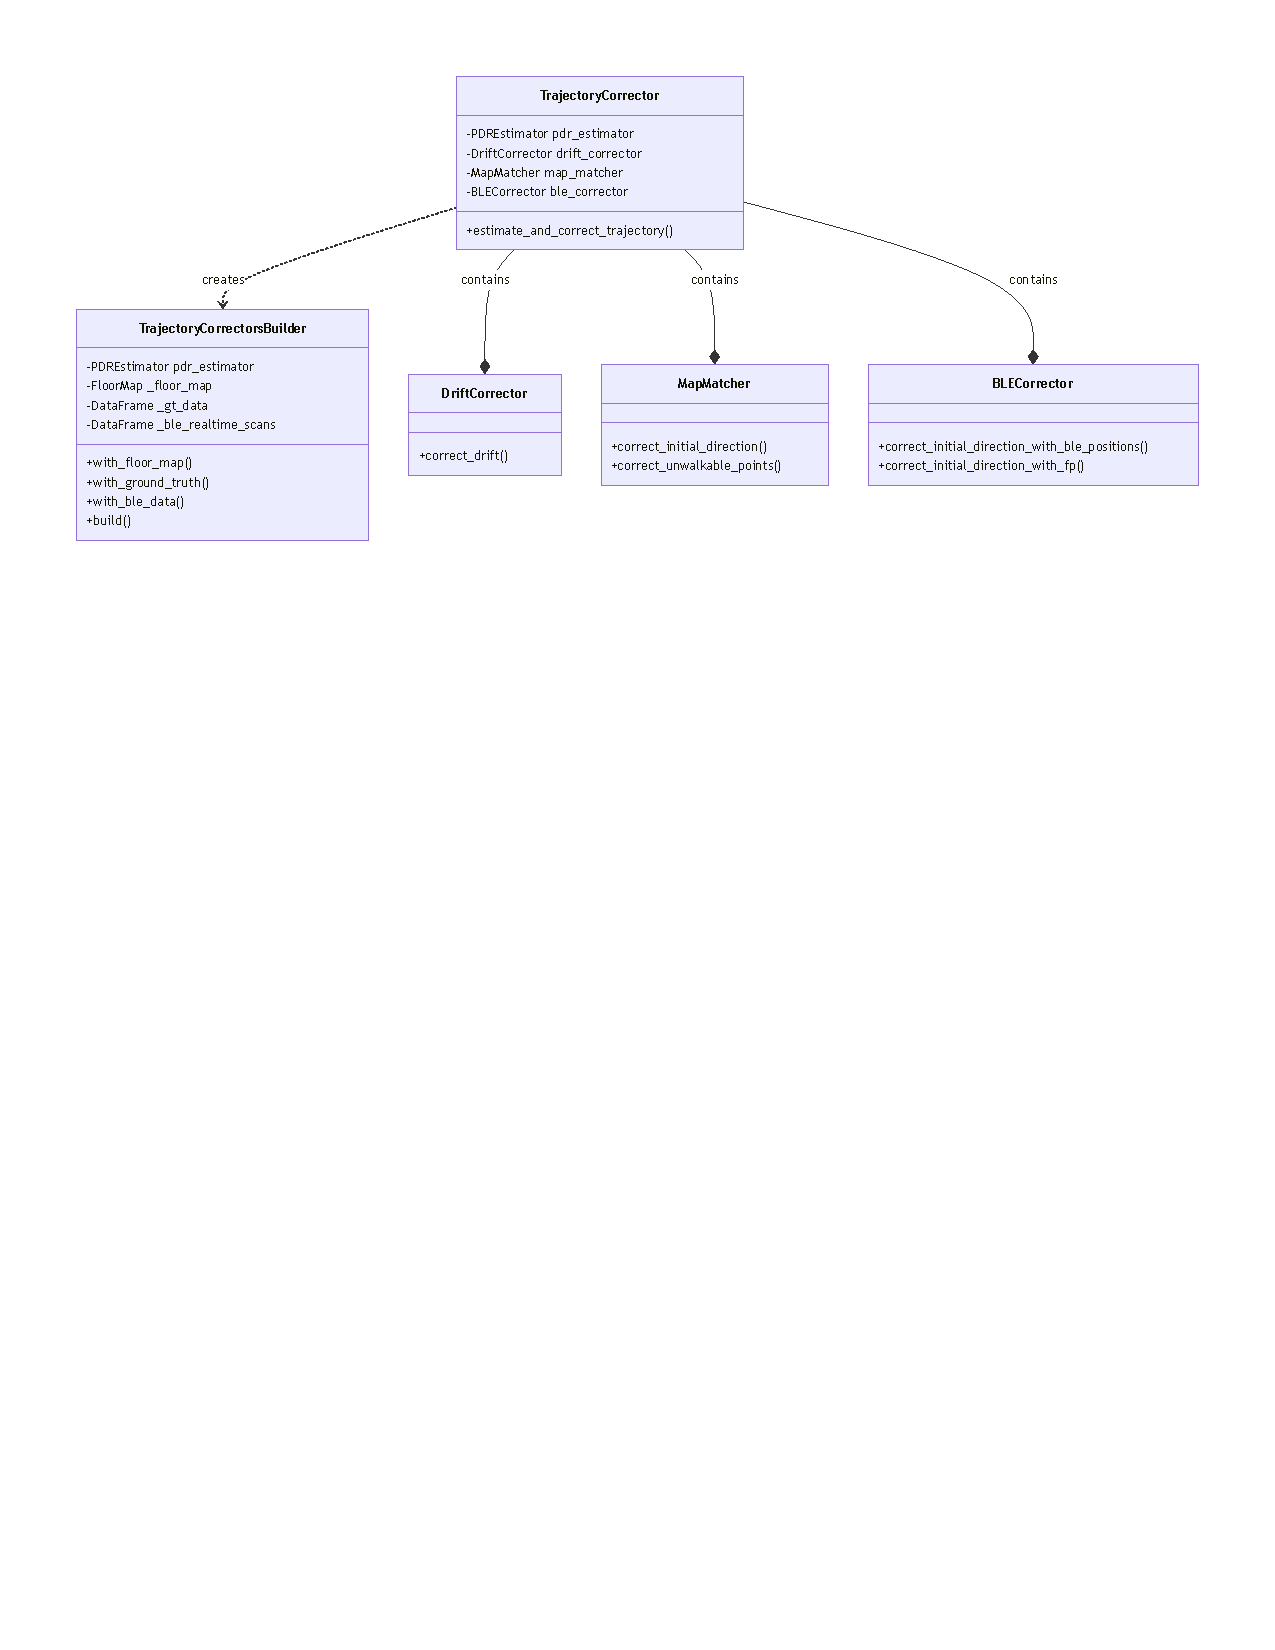
\includegraphics[width=\linewidth]{image/corrector-class-diagram.pdf}
    \caption{補正における主要クラス設計}
    \label{fig:corrector-class}
\end{figure}
% TODO:3.図の文字が小さくて読めない,図を大きくするといいかも



\begin{figure}[H]
    \centering
    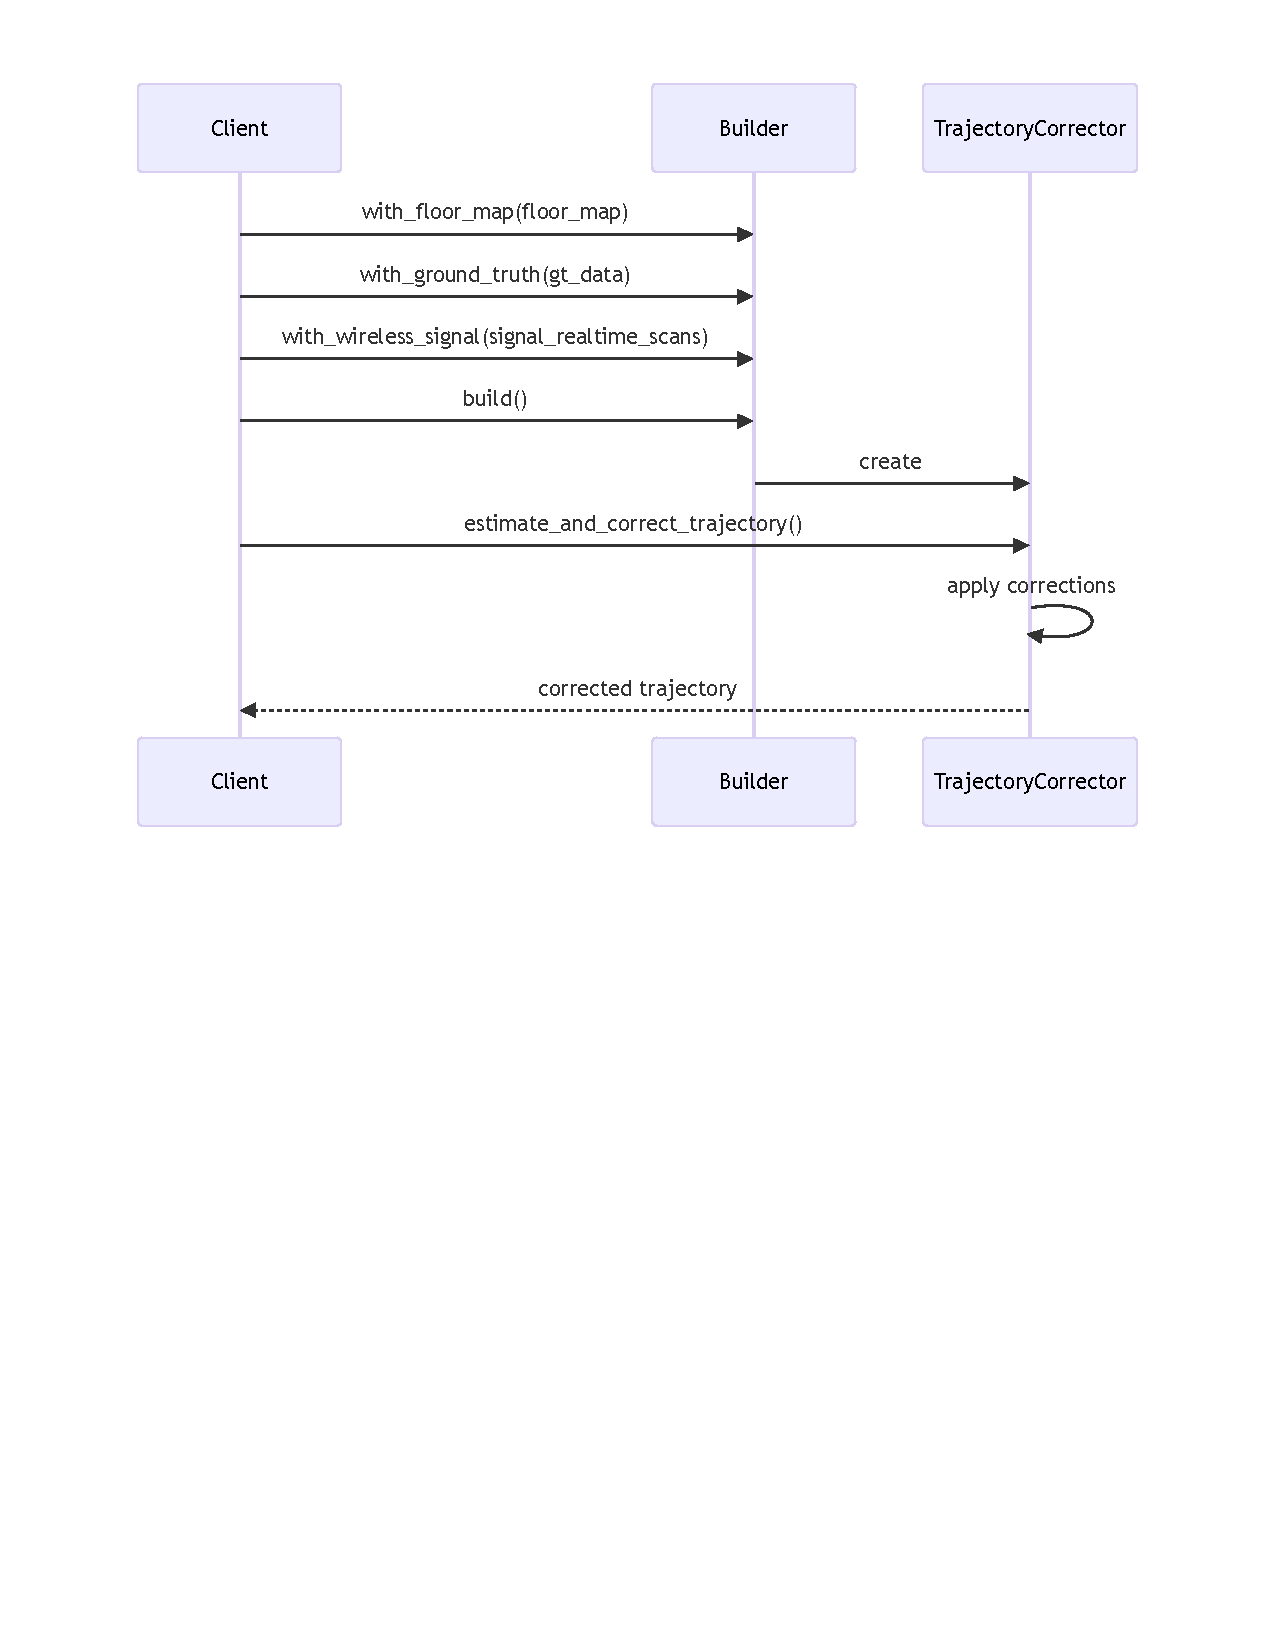
\includegraphics[width=\linewidth]{image/corrector-flow-diagram.pdf}
    \caption{補正の処理フロー}
    \label{fig:corrector-sequence}
\end{figure}
